%% Theorie.tex
%%
%\usepackage[ngerman]{babel}
%% ==============
\chapter{Experimentelle Grundlagen}
\label{ch:experiment}
%% ==============

{\bibliographystyle{babalpha-fl}}	% german style

Zur Untersuchung der theoretischen Vorhersagen des Standardmodells, werden weltweit Experimente durchgef\"uhrt. In Kapitel \ref{ch:experiment} werden die experimentellen Grundlagen anhand des Compact-Muon-Solenoid-Experiment (CMS, Abschnitt \ref{ch:Experiment:sec:CMS}) am Large-Hadron-Collider (LHC, Abschnitt \ref{ch:Experiment:sec:LHC}) des CERN vorgestellt. Anschlie\ss end wird der Ablauf einer Hochenergiephysik-Analyse am Beispiel der \ttH-Analyse vorgestellt.

%% ===========================
\section{Der Large Hadron Collider (LHC)}
\label{ch:Experiment:sec:LHC}
%% ===========================

Der Large-Hadron-Collider (LHC) ist ein Teilchenbeschleuniger der Europ\"aischen Organisation f\"ur Kernforschung (CERN). Er befindet sich in einem 26,7 km langen Tunnel im Grenzgebiet zwischen Frankreich und der Schweiz bei Genf zwischen 45 m und 170 m unter der Erdoberfl\"ache. Es ist der zur Zeit leistungsst\"arkste Teilchenbeschleuniger der Welt.\\
Der LHC kann mit Protonen oder Bleiionen betrieben werden. Wenn Protonen genutzt werden, durchlaufen diese zun\"achst in einer Reihe von Vorbeschleunigern in denen sie pr\"apariert werden. Als erstes wird Wasserstoffgas ionisiert. Die so entstehenden Protonen werden im LINAC2, einem Linearbeschleuniger in B\"undeln (bunches) mit je $1,1\cdot 10^{11}$ Protonen auf 50 MeV beschleunigt \cite{O'Luanaigh:1997427}. Anschlie\ss end werden die Protonenbunches im Proton-Synchrotron-Booster (PSB), im Proton-Synchroton (PS) und im Super-Proton-Synchrotron (SPS) erst auf 1,4 GeV, dann auf 25 GeV und schlie\ss lich auf 450 GeV beschleunigt \cite{O'Luanaigh:1997193}. Im LHC selbst werden in zwei Strahlr\"ohren jeweils maximal 2808 bunches in entgegengesetzte Richtungen auf maximal 7 TeV beschleunigt \cite{Lefevre:1165534}. Die Protonen werden an bestimmten Punkten zur Kollision gebracht. \\
Es gibt sieben Experimente die die bei den Kollisionen entstehenden Teilchen untersuchen. Diese Experimente werden von Kollaborationen von Wissenschaftlern aus aller Welt durchgef\"uhrt. Die beiden gr\"o\ss ten sind ATLAS und CMS, die mit ihren universellen Teilchendetektoren alle entstehenden Kollisionsprodukte untersuchen k\"onnen, w\"ahrend bei dem Schwerionen-Experiment ALICE (A Large Ion Collider Experiment) und dem Large-Hadron-Collider-beauty-Experiment (LHC-B) spezifische Ph\"anomene untersucht werden. ALICE wurde entwickelt um durch Kollisionen von Bleiionen ein Quark-Gluon-Plasma zu erzeugen, was den Bedingungen kurz nach dem Urknall entspricht. LHC-B untersucht Unterschiede zwischen Materie und Antimaterie mithilfe von b-Quarks. Die kleineren Experimente sind TOTEM (Total, elastic and diffractive cross-section measurement) und LHCf (Large Hadron Collider forward), die beide "vorw\"arts" gestreute Ereignisse, also Ereignisse mit sehr kleinem Streuwinkel untersuchen, sowie MoEDAL (Monopole and Exotics Detector at the LHC), das nach magnetischen Monopolen sucht. \cite{O'Luanaigh:1997374, O'Luanaigh:1997265, O'Luanaigh:1997262, O'Luanaigh:1997259, O'Luanaigh:1997373, O'Luanaigh:1997527}\\
In Abbildung \ref{fig:LHC} ist der schematische Aufbau des LHC mit den Experimenten CMS, Atlas, LHC-B und ALICE abgebildet. Die Vorbeschleuniger sind dabei au\ss er dem SPS nicht ber\"ucksichtigt.

\begin{figure}[hhh]
 \begin{center}
   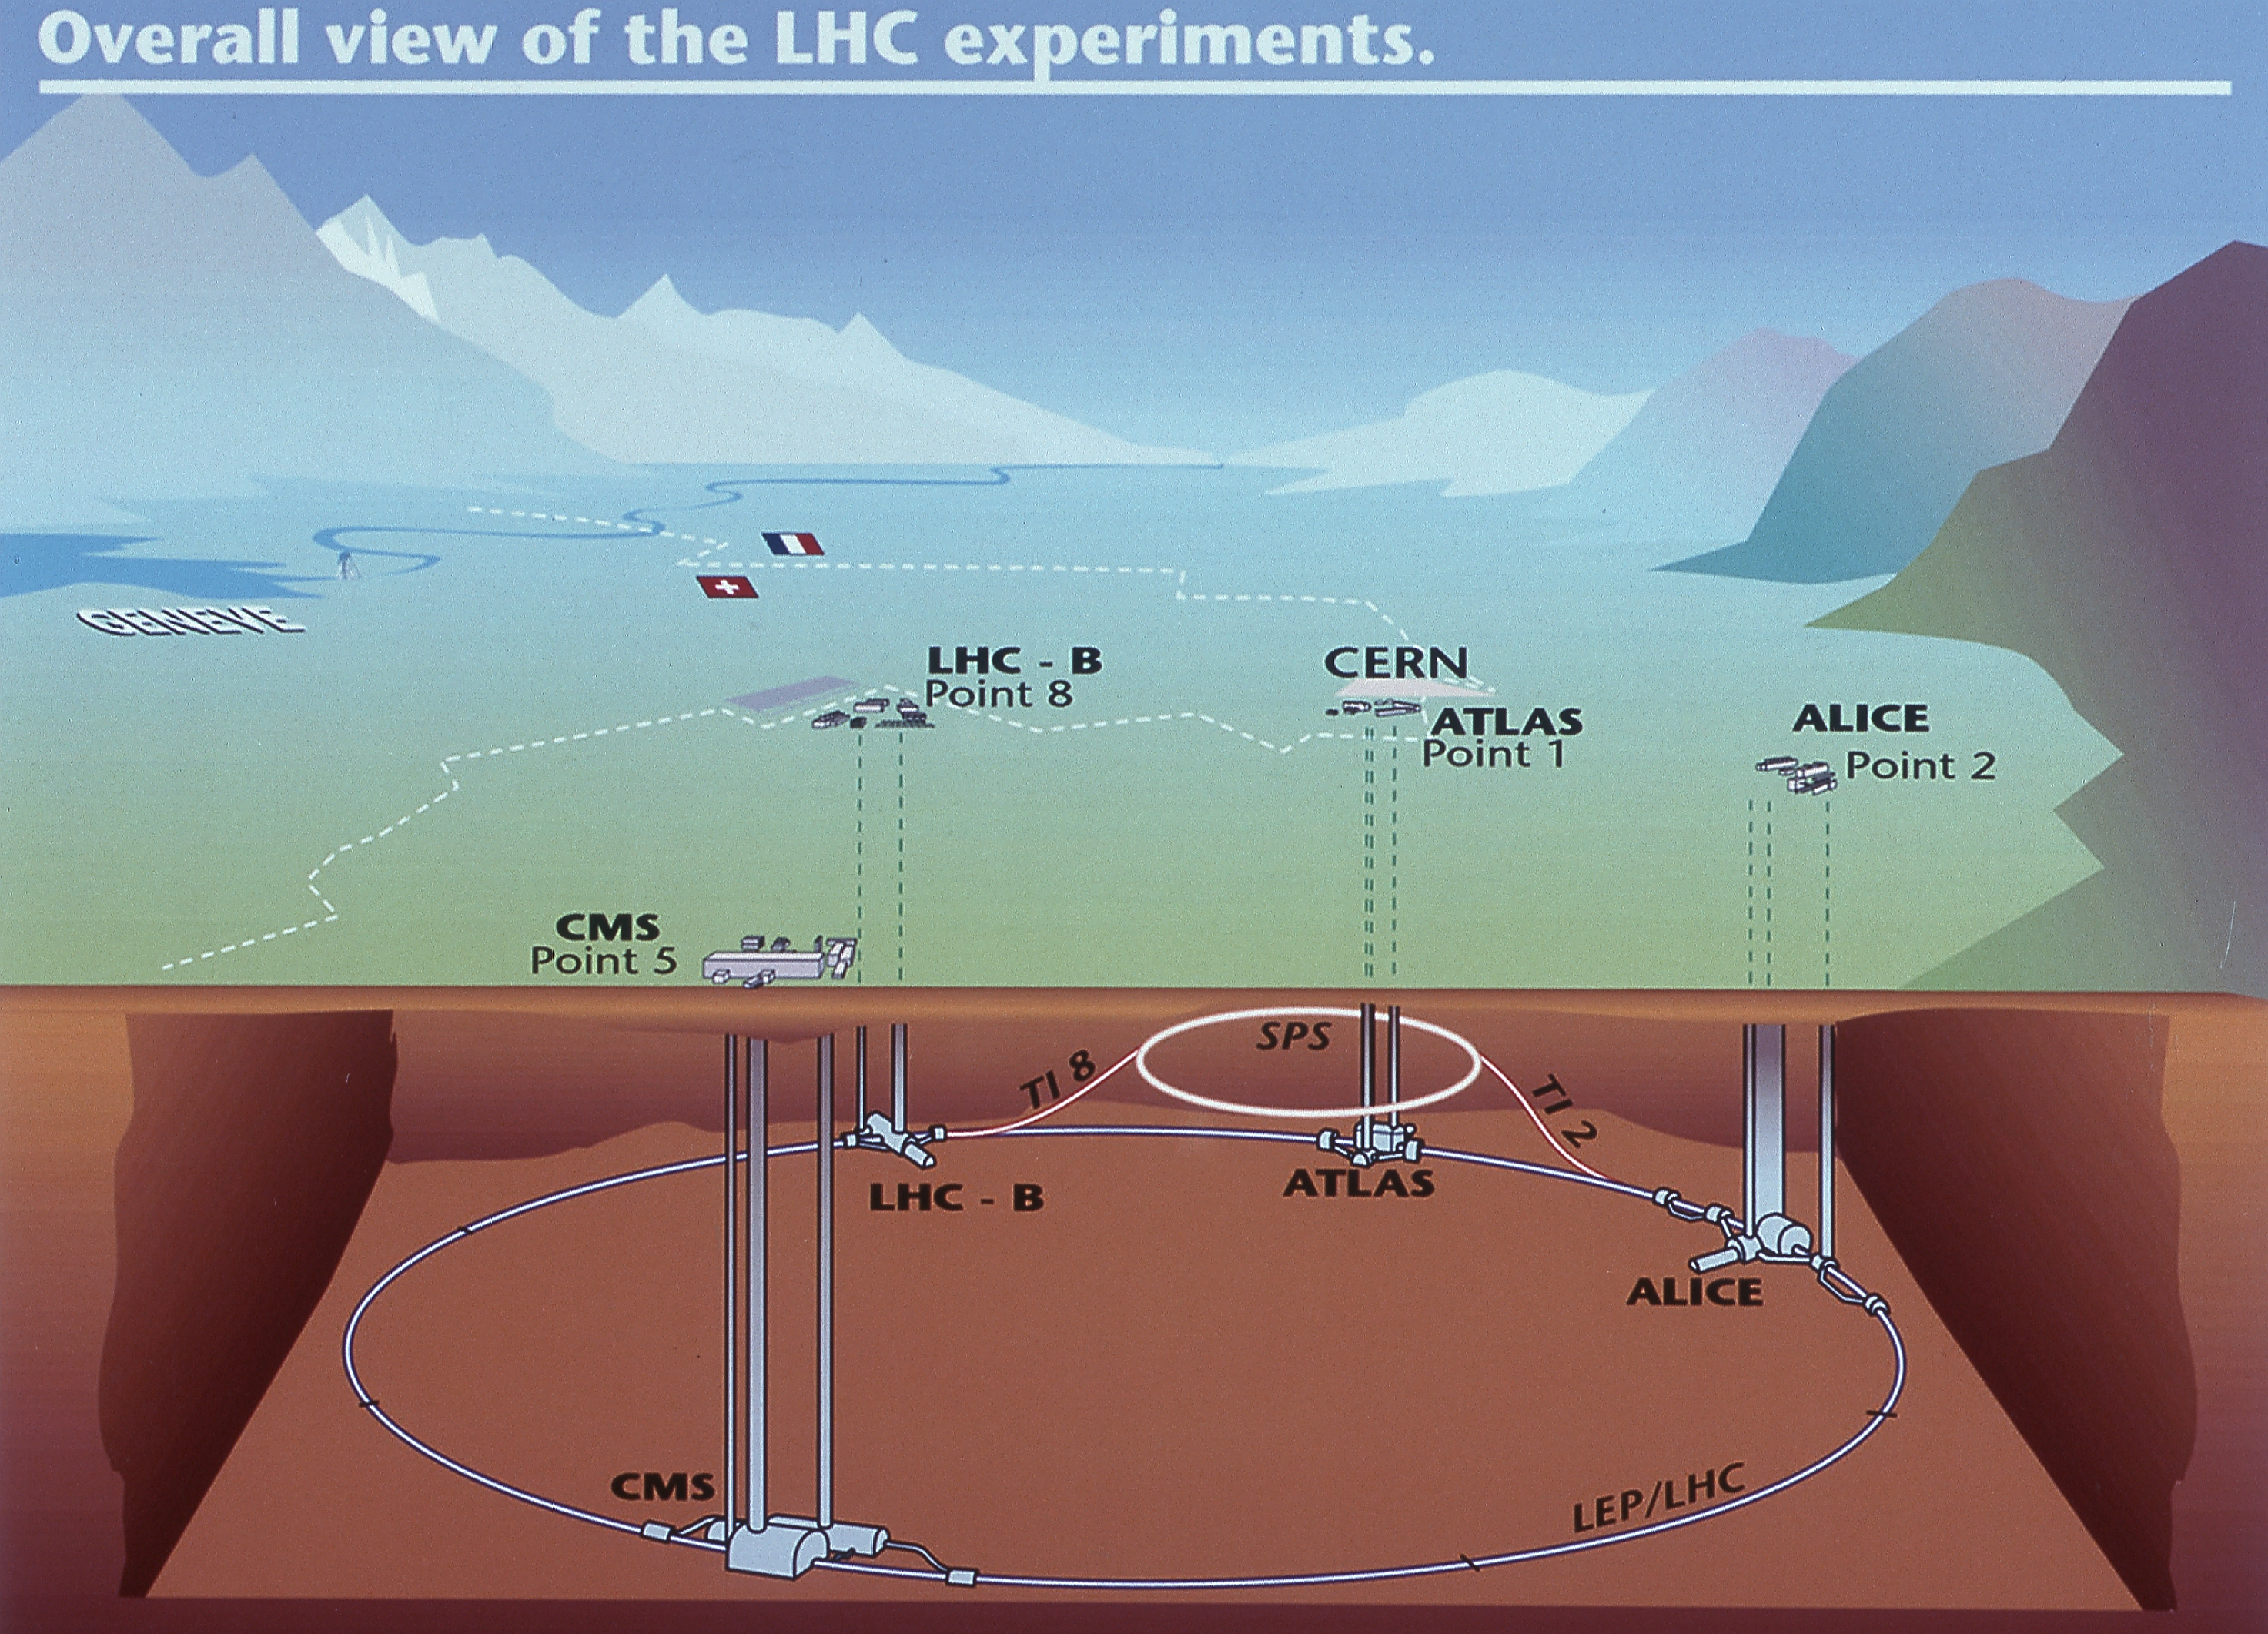
\includegraphics[width=0.8\textwidth]{graphics/LHC_experiments.jpg}
   \parbox[b]{12cm}{
     \caption[Large-Hadron-Collider]
             {\label{fig:LHC} \it\!Der LHC mit den vier Hauptexperimenten und dem Super-Proton-Synchrotron, \cite{Team:40525}}
   }
 \end{center}
\end{figure}

%% ===========================
\section{Der Compact-Muon-Solenoid-Detektor (CMS)}
\label{ch:Experiment:sec:CMS}
%% ===========================



%% ===========================
\section{\ttH-Analyse}
\label{ch:Experiment:sec:ttH}
%% ===========================
